
\chapter{System Design\label{ch:system}}

\section{Quadcopter Characteristics}

    Quadcopters and other multi-rotor aircraft are mechanically much simpler than their conventional rotorcraft counterparts. In order to change roll, pitch, and yaw, a traditional helicopter uses a combination of mechanical linkages changing the pitch of the main rotor blades and a tail rotor. Quadcopters, on the other hand, consist of four fixed-pitch rotors which can be independently controlled to achieve a full range of motion. Because of their mechanical simplicity, Quadcopters are relatively simple to maintain and repair. Additionally, quadcopters are very highly maneuverable due to the ability to rapidly change the thrust of any individual rotor. Also, as there are four rotors contributing to the vertical thrust, each individual rotor possesses less kinetic energy than a single main rotor on a traditional helicopter, making them safer to be used in indoor spaces and around humans. 

    \subsection{Basics of Quadcopter Flight}

        \begin{figure}[ht]
                \centering
                \begin{subfigure}[b]{0.4\textwidth}
                        \centering
                        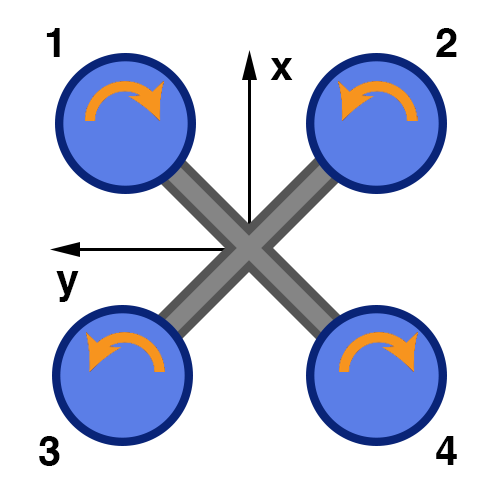
\includegraphics[width=\textwidth]{../images/hover.png}
                        \caption{Hover}
                        \label{fig:hover}
                \end{subfigure}%
                ~ %add desired spacing between images, e. g. ~, \quad, \qquad etc.
                  %(or a blank line to force the subfigure onto a new line)
                \begin{subfigure}[b]{0.4\textwidth}
                        \centering
                        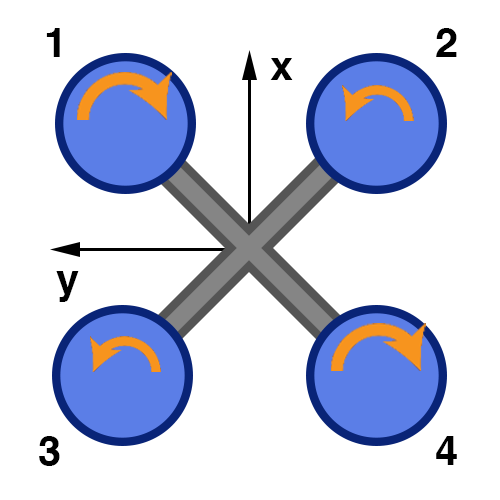
\includegraphics[width=\textwidth]{../images/yaw.png}
                        \caption{Yaw}
                        \label{fig:yaw}
                \end{subfigure}
                \\
                \begin{subfigure}[b]{0.4\textwidth}
                        \centering
                        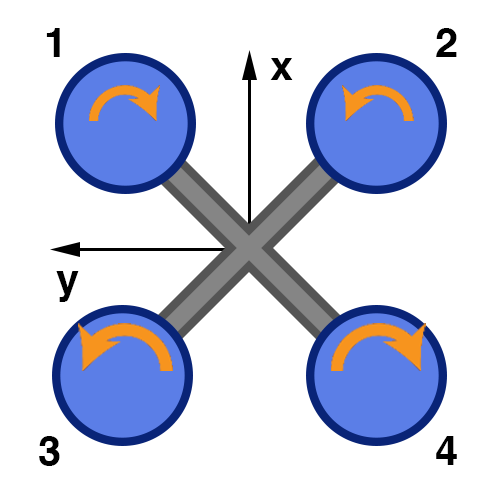
\includegraphics[width=\textwidth]{../images/pitch.png}
                        \caption{Pitch}
                        \label{fig:pitch}
                \end{subfigure}
                ~
                \begin{subfigure}[b]{0.4\textwidth}
                        \centering
                        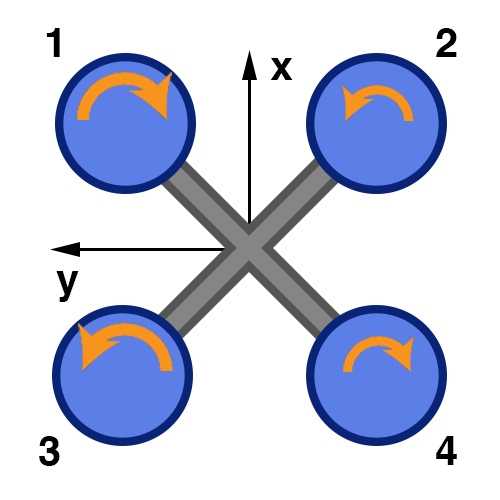
\includegraphics[width=\textwidth]{../images/roll.png}
                        \caption{Roll}
                        \label{fig:roll}
                \end{subfigure}
                \caption{Quadcopter Flight Control.}\label{fig:flightbasics}
        \end{figure}

        Each rotor produces a downwards thrust and torque opposite to the direction of rotation. In order to counter this torque, rotors along a single arm rotate in one direction, with the other rotors rotation in the other direction, as seen in Figure~\ref{fig:flightbasics}. If all of the rotors are turning at the same rate, then the torque forces will cancel out and the quadcopter will hover without rotating (Figure~\ref{fig:hover}). In order to change yaw, two of the rotors spinning in the same direction increase their thrust, and therefore their torque, and the other two rotors slow (Figure~\ref{fig:yaw}). This induces a change in yaw without affecting the overall thrust. In order to change pitch or roll, two rotors on the same side increase thrust, with the other rotors decreasing thrust (Figures~\ref{fig:pitch}~and~\ref{fig:roll})~\cite{Dijkshoorn}.

\section{Parrot AR.Drone 2.0}

    This system will use the AR.Drone 2.0, the second generation of the consumer-grade quadcopter released by Parrot in 2010. The AR.Drone is a stabilized aerial platform that can be controlled by a user-friendly interface on a variety of mobile devices such as the Apple iPhone or iPad. The quadcopter is equipped with cameras and can be used for recording videos and playing augmented reality games.

    \begin{figure}[ht]
            \centering
            \begin{subfigure}[b]{0.5\textwidth}
                    \centering
                    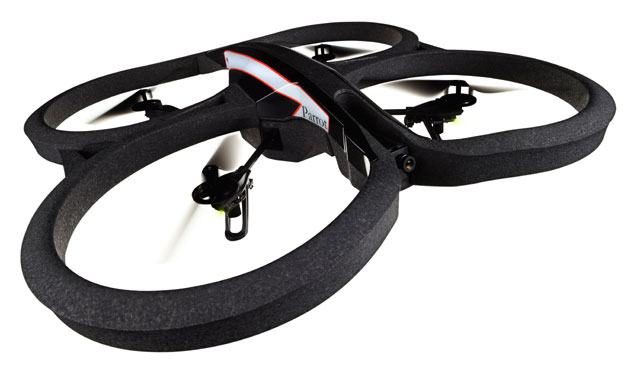
\includegraphics[width=\textwidth]{../images/ardrone_indoor.jpg}
                    \caption{Indoor Hull}
                    \label{fig:indoor}
            \end{subfigure}%
            ~ %add desired spacing between images, e. g. ~, \quad, \qquad etc.
              %(or a blank line to force the subfigure onto a new line)
            \begin{subfigure}[b]{0.5\textwidth}
                    \centering
                    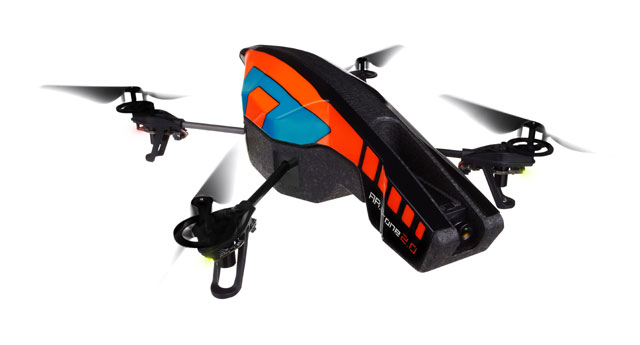
\includegraphics[width=\textwidth]{../images/ardrone_outdoor.jpg}
                    \caption{Outdoor Hull}
                    \label{fig:outdoor}
            \end{subfigure}
            \caption{Parrot AR.Drone 2.0~\cite{ParrotPress}.}\label{fig:ardrone}
    \end{figure}

    \begin{table}
    	\centering
    	\def\arraystretch{1.5} 	
        \begin{tabular}{|l|l|}
        \hline
        Forward Camera          & HD, 720p                                   \\
        ~                       & 92\degree diagonal viewing area            \\ \hline
        Bottom Camera           & QVGA, 320x240                              \\
        ~                       & 64\degree diagonal viewing area            \\ \hline
        Computational Resources & 1 GHz ARM Cortex-A8 CPU                    \\
        ~                       & 800 MHz Video Digital Signal Processor     \\
        ~                       & 256 MB (1 Gbit) DDR2 RAM                   \\ \hline
        Networking              & 802.11n WiFi                               \\ \hline
        Sensors                 & 3-axis gyroscope (2000 degree/second)      \\
        ~                       & 3-axis accelerometer (+/- 50 mg precision) \\
        ~                       & 3-axis magnetometer (6 degree precision)   \\
        ~                       & Pressure sensor (+/- 10 Pa precision)      \\
        ~                       & Ultrasound altitude sensor                 \\ \hline
        \end{tabular}
        \medskip
        \caption{AR.Drone 2.0 Technical Specifications~\cite{Bristeau}.}
    \end{table} 

    \subsection{Features}
        Considering its target audience of consumers, the AR.Drone is actually a very powerful research platform. The quadcopter is ready-to-fly out of the box. Unlike most quadcopters which are sold as kits, there is no assembly or technology knowledge needed to get started. Additionally, with the provided SDK, it is relatively easy to get off the ground and start running code to control the quadcopter. Finally, at only \$300, the AR.Drone is much easier to fit into most research budgets than kit quadcopters which can cost thousands of dollars. 

        The AR.Drone has two cameras, one forward-facing HD camera, and one lower resolution high frame-rate camera facing downwards. The AR.Drone processes the visual imagery on board to produce a velocity estimate. Depending on the ground material and lighting quality, the AR.Drone uses either muti-resolution optical flow or FAST corner detection with least-squares minimization. The drone also uses the gyroscope and accelerometer on the navigation board to produce a velocity estimate and fuses this estimate with the vision-based velocity to create a relatively robust velocity estimation~\cite{Bristeau}. %CHECK TO SEE IF THIS IS TRUE

        For altitude estimation, the AR.Drone uses a combination of an ultrasonic range sensor and pressure sensor. At heights under 6 meters, the AR.Drone relies solely on the ultrasonic sensor. Above those heights, where the ultrasonic sensor is not in its operational range, the AR.Drone estimates altitude based on the difference between the current pressure and the pressure measured on takeoff. 

        The on-board processor handles low-level stabilization and wind compensation, allowing the quadcopter to hold position when not receiving control inputs. Commands to the AR.Drone are sent in the form of desired pitch and roll angles for translational movements, angular rate for yaw adjustment, and velocity for altitude adjustments. These high level commands are then translated by the on-board controller into rotor speed adjustments. Typically difficult actions, such as takeoff and landing, are completely handled by the onboard control. When the takeoff command is issued, the AR.Drone quickly takes off to a default height and hovers before accepting any movement commands.

    \subsection{Limitations}

        While the AR.Drone is a great platform for many research projects, it does have limitations when compared to hobbyist or professional-grade quadcopters.

        The hardware design allows for very little customization. While most professional-grade quadcopters have ports for adding additional sensors, there is no straightforward way to add any electronics to the AR.Drone. Even if it were possible to customize, the AR.Drone is designed to only lift its own weight, with most hobbyists claiming to get a maximum of 100 grams payload before the flight characteristics are significantly affected~\cite{Forums}. Professional quadcopters of a similar size are typically able to fly with payloads between 400 and 600 grams~\cite{Mikrocopter}.

        Another limitation of the AR.Drone is the flight time. The maximum flight time of the AR.Drone is only around 15 minutes, with the additional weight of the indoor hull bringing this down to 10-12 minutes. Similar sized quadcopters, such as the Mikrocopter, typically achieve around 30 minutes of flight time, depending on weight and battery size~\cite{Mikrocopter}.

        Additionally, the AR.Drone has no built in GPS system, meaning that the on board measurements provide only relative measurements. This leads to errors in drift and makes flying autonomously in a precise pattern an extremely challenging task.

        Finally, as the AR.Drone was designed to be used by inexperienced pilots, extra emphasis was put on making the quadcopter durable when it is inevitably crashed. Due to this, the polystyrene case and hull, particularly the indoor hull, around the body are much larger than that of the Mikrocopter or similar quadcopters. This results in a larger surface area that can be affected by the wind, making outdoor flights particularly difficult even with the on board stabilization. 

\section{System Architecture}

    \begin{figure}[ht]
            \centering
            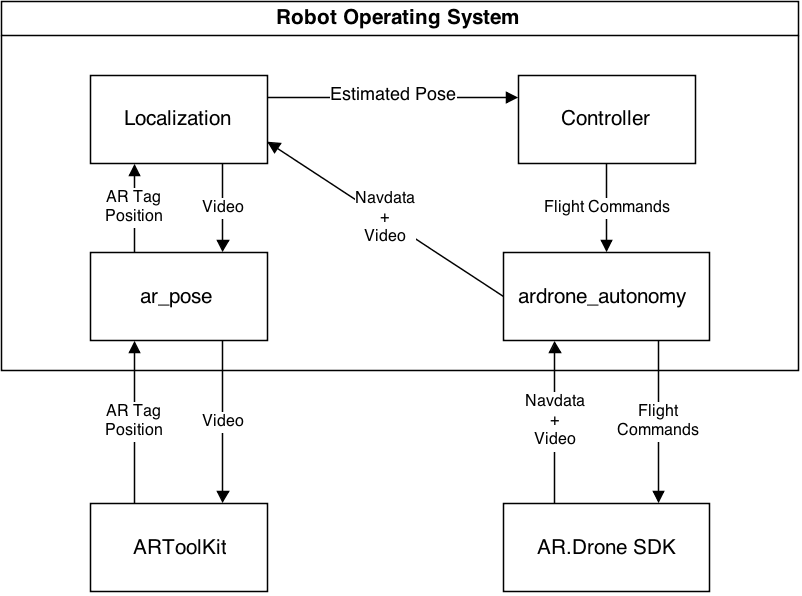
\includegraphics[width=400px]{../images/system.png}
            \caption{System Architecture Diagram.}\label{fig:system}
    \end{figure}

    \subsection{Robot Operating System}
         The Robot Operating System (ROS) is used to organize the interaction between programs and libraries. Although not an ``operating system'' in the traditional sense, ROS is an open source communication layer used in a wide variety of robotics applications. Supported by Willow Garage, ROS has a large amount of documentation and packages which can handle a large number of common tasks in robotics. Many of these packages are hardware-independent, meaning that they can be quickly implemented on an array of different robotics system. ROS also provides a standard message protocol, allowing packages to work together in a language agnostic manner~\cite{ROS}.

    \subsection{ardrone\_autonomy}
        ``ardrone\_autonomy'' is an open-source ROS wrapper for the Parrot AR.Drone SDK developed in the Autonomy Lab at Simon Fraser University~\cite{Autonomy}. This package handles the interface of navdata messages, video feeds, and control commands between ROS and the AR.Drone. This allows the use of many existing ROS packages in localizing and controlling the quadcopter.

    \subsection{ARToolKit}
        ARToolKit is an open-source software library designed to be used for creating Augmented Reality applications. Developed by Dr. Hirokazu Kato and maintained by the HIT lab at the University of Washington, ARToolKit uses computer vision algorithms to identify fiduciary markers, such as the one in Figure ~\ref{fig:artag}, and calculate the transformation between camera and tag orientation. 

        For augmented reality applications, this can be used to superimpose 3D graphics onto a video feed in real time based on the tag position and orientation. In this system, the tags will be used to generate global positioning estimates for the quadcopter by combining estimated tag transformations with known tag locations.

        Specifically, ARToolKit will be implemented using a slightly modified version of the ar\_pose library, a ROS wrapper for ARToolKit developed by Ivan Dryanovski et al. at the CCNY robotics lab~\cite{arpose}.

        \begin{figure}[ht]
                \centering
        		
\includegraphics[width=200px]{../images/artag.png}
                \caption{Augmented Reality Tag With ID 42.}\label{fig:artag}
        \end{figure}


    \subsection{Localization}
        The purpose of the localization module is to produce an estimated pose of the quadcopter. The localization module receives navdata and the video feed from AR.Drone via ardrone\_autonomy. Localization then sends the video to the ar\_pose to get any augmented reality tag transformations. Then, using a combination of sensor data from the navdata message and tag transformations from ar\_pose, localize then produces an updated estimated pose.

    \subsection{Controller}
        % Mention Sarah!
        The purpose of the controller is to produce the control inputs in order to move the quadcopter from its current pose to a desired pose. The controller receives the estimated pose from the localization module and sends the flight commands to ardrone\_autonomy.

    \subsection{3D Reconstruction Software}
        After the flight is complete, 3D reconstruction software is used to turn the collection of images into a 3D model. There are multiple off the shelf libraries, including open-source Clustering Views for Muti-view Stero (CVMS) and commercial Agisoft Photoscan~\cite{CMVS, Agisoft}. 

